% Simplified attribution graph visualisation
% Side-by-side: Gemma-2-2B (26 layers) and Llama-3.2-1B (16 layers)
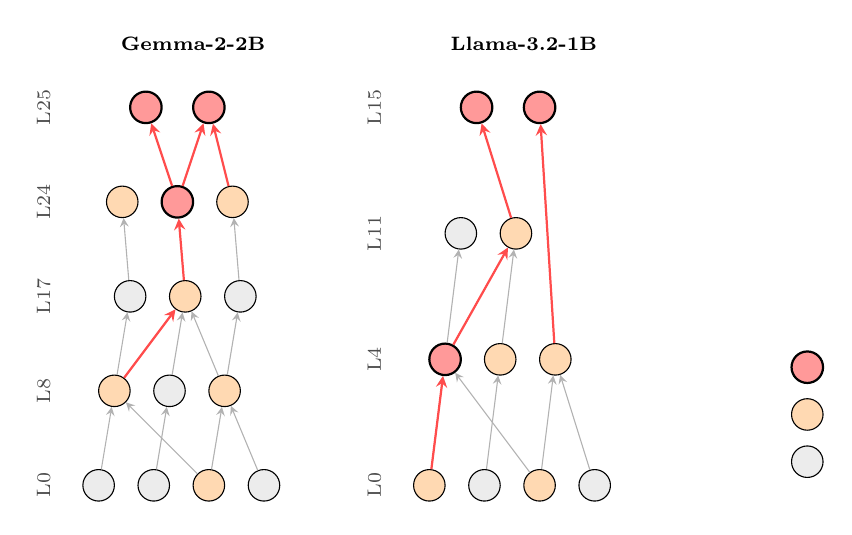
\begin{tikzpicture}[
  node distance=0.6cm and 1.2cm,
  feat/.style={circle, draw, minimum size=0.4cm, inner sep=0pt, font=\tiny},
  high/.style={feat, fill=red!40, thick},
  med/.style={feat, fill=orange!30},
  low/.style={feat, fill=gray!15},
  edge/.style={->, >=stealth, thin, gray!60},
  strong/.style={->, >=stealth, thick, red!70},
  label/.style={font=\scriptsize, text=black!70},
  ptitle/.style={font=\scriptsize\bfseries, anchor=south},
]

% --- Gemma-2-2B (left) ---
\node[ptitle] at (1.2, 5.4) {Gemma-2-2B};
\node[label, rotate=90] at (-0.7, 0) {L0};
\node[label, rotate=90] at (-0.7, 1.2) {L8};
\node[label, rotate=90] at (-0.7, 2.4) {L17};
\node[label, rotate=90] at (-0.7, 3.6) {L24};
\node[label, rotate=90] at (-0.7, 4.8) {L25};

\node[low] (g00) at (0, 0) {};
\node[low] (g01) at (0.7, 0) {};
\node[med] (g02) at (1.4, 0) {};
\node[low] (g03) at (2.1, 0) {};

\node[med] (g10) at (0.2, 1.2) {};
\node[low] (g11) at (0.9, 1.2) {};
\node[med] (g12) at (1.6, 1.2) {};

\node[low] (g20) at (0.4, 2.4) {};
\node[med] (g21) at (1.1, 2.4) {};
\node[low] (g22) at (1.8, 2.4) {};

\node[med] (g30) at (0.3, 3.6) {};
\node[high] (g31) at (1.0, 3.6) {};
\node[med] (g32) at (1.7, 3.6) {};

\node[high] (g40) at (0.6, 4.8) {};
\node[high] (g41) at (1.4, 4.8) {};

\draw[edge] (g00) -- (g10);
\draw[edge] (g01) -- (g11);
\draw[edge] (g02) -- (g10);
\draw[edge] (g02) -- (g12);
\draw[edge] (g03) -- (g12);
\draw[edge] (g10) -- (g20);
\draw[edge] (g11) -- (g21);
\draw[edge] (g12) -- (g21);
\draw[edge] (g12) -- (g22);
\draw[edge] (g20) -- (g30);
\draw[edge] (g22) -- (g32);
\draw[strong] (g10) -- (g21);
\draw[strong] (g21) -- (g31);
\draw[strong] (g31) -- (g40);
\draw[strong] (g31) -- (g41);
\draw[strong] (g32) -- (g41);

% --- Llama-3.2-1B (right) ---
\begin{scope}[xshift=4.2cm]
\node[ptitle] at (1.2, 5.4) {Llama-3.2-1B};
\node[label, rotate=90] at (-0.7, 0) {L0};
\node[label, rotate=90] at (-0.7, 1.6) {L4};
\node[label, rotate=90] at (-0.7, 3.2) {L11};
\node[label, rotate=90] at (-0.7, 4.8) {L15};

\node[med] (l00) at (0, 0) {};
\node[low] (l01) at (0.7, 0) {};
\node[med] (l02) at (1.4, 0) {};
\node[low] (l03) at (2.1, 0) {};

\node[high] (l10) at (0.2, 1.6) {};
\node[med] (l11) at (0.9, 1.6) {};
\node[med] (l12) at (1.6, 1.6) {};

\node[low] (l20) at (0.4, 3.2) {};
\node[med] (l21) at (1.1, 3.2) {};

\node[high] (l30) at (0.6, 4.8) {};
\node[high] (l31) at (1.4, 4.8) {};

\draw[edge] (l00) -- (l10);
\draw[edge] (l01) -- (l11);
\draw[edge] (l02) -- (l10);
\draw[edge] (l02) -- (l12);
\draw[edge] (l03) -- (l12);
\draw[edge] (l10) -- (l20);
\draw[edge] (l11) -- (l21);
\draw[strong] (l00) -- (l10);
\draw[strong] (l10) -- (l21);
\draw[strong] (l21) -- (l30);
\draw[strong] (l12) -- (l31);
\end{scope}

% Legend
\node[low, label=right:{\tiny Low}] at (9.0, 0.3) {};
\node[med, label=right:{\tiny Moderate}] at (9.0, 0.9) {};
\node[high, label=right:{\tiny High}] at (9.0, 1.5) {};

\end{tikzpicture}
